\chapter{Analysis Pipeline}\label{chap:pipeline}
%%%Talk in more detai about data taken. Explain how data at 3100 is treated (calibration, cuts...) and refer to undepleted section for other voltages.
Compton data were taken along the $\left<1\,0\,0\right>$ (fast) and $\left<1\,1\,0\right>$ (slow) axis of the ICPC, at operating (3500\,V) and near-operating (3100\,V) bias. The fast axis scan at operating bias was chosen as a high statistics run, with 2-3 times more data taken than in the other configurations. The near-operating bias was chosen as representative of how some detectors are currently operated in the LEGEND-200 experiment, where full depletion, but not operating bias is reached. In such detectors, increases in leakage current or HV discharges prevents the operation at full bias. Thus, the study of an ICPC detector under near-operating bias is warranted. All Compton data were processed in 4 tiers, with the optimal goal of creating a pulse shape library. 
\begin{itemize}
	\item Tier 0 Filter: As described in Sec.~\ref{sec:daq}, raw Compton data was filtered in parallel to data acquisition. In this process, only events coincident between the detector and camera were saved.
	\item Tier 1 Process: The waveform parameters described in Chapter~\ref{chap:param} were calculated for all filtered events. 
	\item Tier 2 Reconstruct: Data cleaning and event selection were conducted based on the Tier 1 waveform parameters. $z$-position was reconstructed for the selected events. The soft-pileup and resting baseline data streams were mixed together at this point; however, their tags were retained and used where relevant, such as in energy resolution dependent calculations and $AvsE$ computation.
	\item Tier 3 Superpulse: Reconstructed events within a $z$-range were combined into a superpulse. Superpulses built in this tier populate the pulse shape library for the ICPC.
\end{itemize}
In this chapter Tier 2 and 3 procedures are outlined using data taken at $r = 31$\,mm during the high statistics fast axis scan. 

\section{Crystal Axis Orientation from Near Surface Events}\label{sec:crystal_axis_Ba}
To pinpoint the fast and slow axes of the detector a dedicated surface scan was performed with a collimated \BaS{} source. Data were taken with the source illuminating a spot approximately 4.3\,mm from the bottom of the detector in the same configuration as used for the ICPC - camera alignment (Fig.~\ref{fig:czt_icpc_alignment_pictures}). This position was determined by pointing the source at the camera, fitting the resulting beam spot, and then moving the source a known vertical distance. The camera beam spot has a FWHM of 3.81\,mm with the collimator aperture approximately 5\,cm from a CZT crystal along the beam path. A similar beam spot diameter is expected on the detector. The detector was scanned azimuthally every 5$^\circ$ at the same height. For each angle, events with no hard or soft pileup in the 81\,keV peak were selected. 
\begin{figure}[H]
    \centering
    \includegraphics[width=6in]{figs/pipeline/Ba_superpulse.png}
    \caption{The \BaS{} spectrum is shown at the top with the selected 81\,keV events shown in red. All pileup free events in the energy window were used to construct the superpulse shown in black below. Note that the superpulse includes small contributions from slow pulses originating at the n$^+$ contact (blue and green waveforms which did not reach the full rise in the time window shown).}
    \label{fig:Ba_superpulse}
\end{figure}

The mean free path of 81\,keV gammas is approximately 2.19\,mm in Ge~\cite{NIST}. This mean free path is ideal for crystal axis determination of an in-cryostat detector, ensuring that gammas can transverse the cryostat wall and the n$^+$ dead layer while restricting energy depositions to a small volume near the surface. The latter allows for the construction of superpulses, which mitigates the poor signal-to-noise ratio at 81\,keV. This is of particular importance for the determination of signal rise time. To create the \BaS{} superpulses, events are time aligned at 50\% of their rise and averaged. This procedure is exemplified in Fig.~\ref{fig:Ba_superpulse}. 

The \BaS{} crystal axis data were taken before the noise upgrade, therefore a large noise amplitude is present. Since the 50\% rise point is determined by a threshold crossing of raw waveforms -- and thus subject to noise -- the superpulse is biased towards higher values at the alignment point. For this reason a kink is observed in the superpulse at 8000\,ns, the chosen alignment time. This effect is expected to average out far from the alignment point, such as at the 1\% and 99\% rise points marked by dotted lines in the bottom panel of the figure. These values are determined by threshold crossings of the superpulse, and their difference is taken to be the 1-99\% rise time. This process is repeated at every angle where approximately 8500 events were used to construct each superpulse. The resulting 1-99\% rise times are shown in Fig.~\ref{fig:crystal_axis_Ba}.  
\begin{figure}[htb]
    \centering
    \includegraphics[width=6in]{figs/pipeline/crystal_axis_Ba.pdf}
    \caption{The 1-99\% rise times are determined as described in the text and shown in gray. The data is fit the sinusoidal function shown in red to determine the crystal axis orientation. The slow and fast axis are extracted from the fit and shown as dashed and dotted vertical lines respectively. A period of 90$^\circ$ is observed as expected.}
    \label{fig:crystal_axis_Ba}
\end{figure}

A sinusoidal fit is performed to the rise time data, determining a 1-99\% rise time anisotropy of $(18.0\pm0.9)$\,ns and locating the slow axis at rotational motor coordinate $\phi = (24.9\pm1.2)^\circ$. A similar measurement was performed with the \BaS{} source placed 80\,mm higher. For this measurement no anisotropy in rise time was found. Based on these results the detector was scanned at $\phi = 24.9^\circ$ and $\phi = 69.9^\circ$ to collect slow and fast axis data respectively.

\section{Event Selection}

The creation of superpulses allowed for the measurement of a 18.0\,ns 1-99\% rise time anisotropy in the \BaS{} data presented. Measuring such a small effect would have not been possible on individual events, whose noise levels and 4\,ns sample length obscure waveform features. Gamma depositions were confined to a small volume at the chosen gamma energy, leading to events with approximately the same shape. When building superpulses from Compton events, this assumption is only as good as the accuracy of the position reconstruction. Therefore, the unbiased selection of events is paramount to ensure reliable superpulses. In this section, the process of selecting a subset of events with one and/or two hits in the camera (referred to as 1- and 2-hit events) is discussed. 

The position of the source ($r$) and camera ($z_\text{CAM}$) for the high statistics fast axis scan is shown in Fig.~\ref{fig:scan_schematic}. These are also shown directly on the pictogram of Fig.~\ref{fig:cleaningcut_stability}. In both figures each multicolored dot represents a saved filtered data file, containing 5\,min of data. 
\begin{figure}[htb]
    \centering
    \includegraphics[width=6in]{figs/pipeline/scan_schematic.pdf}
    \caption{Location or the \CsS{} source and camera in the detector coordinate system during the high statistics fast axis scan of the detector. LN$_2$ fills are shown in pink.}
    \label{fig:scan_schematic}
\end{figure}
To cover the entire bulk of the detector, which extends 99.8\,mm in $z$-axis, the camera was placed in up to 4 different locations in $z$ for each radial position of the source. In addition, the detector is scanned at 2\,mm intervals in $r$ starting at the outer edge of the detector and finishing at 1\,mm from the center. This interval is chosen to approximately match the average \CsS{} beam spot diameter throughout the detector, thus ensuring that the entire detector is illuminated. Measurement time was increased with decreasing $r$, to compensate for increased scattered gamma attenuation and decreased solid angle coverage by the camera. A similar scanning profile was employed for all other radial scans.  

In addition to removing events captured during LN$_2$ fills, three data cleaning cuts are applied to filtered data in Tier 2 processing: hard pileup, burst, slope-offset. These are based on the parameters described in Chapter~\ref{chap:param}. The slope-offset cut discards the events which do not fall in the resting baseline or soft pileup regions in the slope-offset space shown in Fig.~\ref{fig:soft_pileup}. The survival fractions of the three data cleaning cuts is shown over time in Fig.~\ref{fig:cleaningcut_stability}.
\begin{figure}[htb]
    \centering
    \includegraphics[width=6in]{figs/pipeline/cleaningcut_stability.pdf}
    \caption{Survival of the three dating cleaning cuts described in the text over time. The pictogram shows the radial position of the \CsS{} source and the $z$-position of the top of the camera as red dots on the detector.}
    \label{fig:cleaningcut_stability}
\end{figure}

The hard pileup survival correlates with the \CsS{} source position as expected, with the positions that led to the highest event rates having the lowest survival fractions. Since the resting baseline and soft pileup event classifier depends on baseline stability, which in turn also depends on rate, a small correlation between slope-offset cut survival and radial position of the source is also observed. This is not the case for the burst cut survival. Burst abundance is suspected to depend on environmental sources of noise, such as equipment in the lab being shut on and off. However, no specific source of noise was pinpointed, and the data are characterized by periodic jumps in burst abundance. 

Events for which the energy is fully deposited within the detector and camera -- contained events -- are selected from ``clean'' data. This is done by selecting events in the 662\,keV sum energy peak as shown on the left of Fig.~\ref{fig:z_reconstruction_energy} and specified by Eq.~\ref{eq:contained_cut}:
\begin{equation}
	\left|E_\text{CAM} + E_\text{IC} - 662\,\text{keV}\right| \leq 8\,\text{keV}~
	\label{eq:contained_cut}
\end{equation}
where $E_\text{IC}$ is the calibrated ICPC energy. The cut is also visualized in the two-dimensional histogram on the right of the figure, where contained events form a strong diagonal. Events under the diagonal are predominantly Compton events which were not fully contained, while events over the diagonal are most likely accidental coincidences. Thus, a stark difference in the number of events under and over the diagonal exists. The camera and detector energy threshold are also visible, at approximately 50\,keV and 100\,keV respectively. 
\begin{figure}[htb]
    \centering
    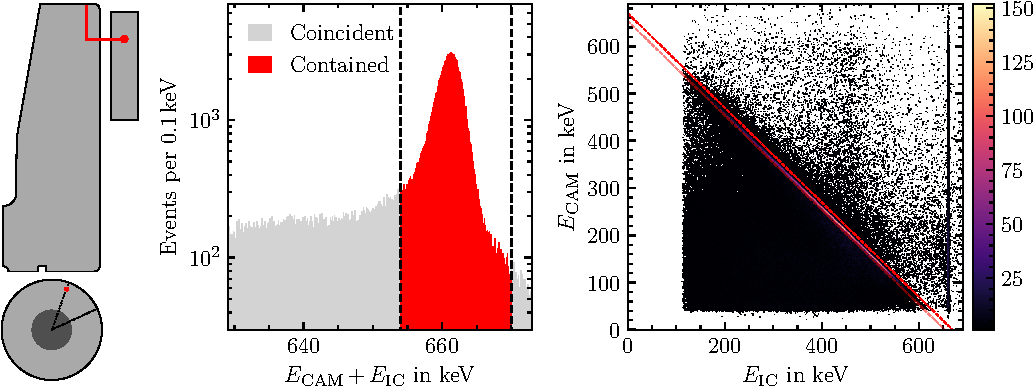
\includegraphics[width=6in]{figs/pipeline/z_reconstruction_energy.png}
    \caption{The sum energy peak and contained cut from Eq.~\ref{eq:contained_cut} is shown on the left. The events in the peak in red are the same as those in between the dashed red lines in the two-dimensional histogram on the right.}
    \label{fig:z_reconstruction_energy}
\end{figure}

1- and 2-hit events were selected from the contained events. For both populations the Compton angle, $\theta$, was calculated with Eq.~\ref{eq:compton}, which is repeated below in terms of the relevant energies for convenience:
\begin{equation} \label{eq:compton_IC}
    \cos(\theta) = 1 - \dfrac{m_ec^2 E_\text{IC}}{662\,\text{keV} \times \left(662\,\text{keV} - E_\text{IC}\right)}~.
\end{equation}
The Compton angle, camera hit position $(x_c,y_c,z_c)$ and \CsS{} source position $(x_0,y_0)$ were used to reconstruct the detector $z$-position, $z_\theta$, via Eq.~\ref{eq:ztheta}, also repeated here. 
\begin{equation} \label{eq:ztheta_IC}
	z_\theta = z_c + \sqrt{(x_c-x_0)^2 + (y_c-y_0)^2} \;\cot(\theta)~. 
 \end{equation}
For 2-hit events -- the subdominant population -- the $\alpha$-reconstruction procedure outlined in Sec.~\ref{sec:workingprinciple} was applied to determine the order of camera hits and validate $z_\theta$. The validation uses the topology and energy of hits in the camera to project a virtual cone which represents the physically allowed gamma paths. Given the superior energy resolution of the detector, the left-hand-side expression of Eq.~\ref{eq:compton_alpha} is used. If the intersection of this cone with the beam axis ($z_\alpha$) was within 2\,mm of $z_\theta$, the reconstruction was considered validated. The fraction of 2-hit events that passed $\alpha$-validation is shown if Fig.~\ref{fig:compton_stability} along the contained event fraction. 
\begin{figure}[htb]
    \centering
    \includegraphics[width=6in]{figs/pipeline/compton_stability.pdf}
    \caption{Contained event fraction was calculated as the number of events which satisfy the relation in Eq.~\ref{eq:contained_cut} to the number of clean coincident events. From these, 2-hit events were selected. The fraction of 2-hit events that passed $\alpha$-validation is shown in the bottom panel. Since both fractions depend on the geometry of the detector camera and source, a dependency on the camera and source position is present.}
    \label{fig:compton_stability}
\end{figure}

Although no secondary validation of $z_\theta$ exists for 1-hit events, events above the 477\,keV Compton shoulder are automatically ruled out by the following constraint imposed by Eq.~\ref{eq:compton_IC}:
\begin{equation}
	\left|1 - \dfrac{m_ec^2 E_\text{IC}}{662\,\text{keV} \times \left(662\,\text{keV} - E_\text{IC}\right)}\right| \leq 1~.
\end{equation}
The detector often extended far below the bottom of the camera. In such cases, events with very obtuse Compton angles are possible. As the angle approaches 180$^\circ$ the small uncertainty in energy translates to a high uncertainty in $\theta$. This effect is compounded by $\cot(\theta)$, which diverges at 180$^\circ$. The combination of these effects led to a large uncertainty in $z_\theta$. Since the energy resolution of the detector is known at all energies for soft pileup and resting baseline events (Fig.~\ref{fig:fwhm_peaks}), the uncertainty in $z_\theta$ can be determined on an event-by-event basis. Events with a $z_\theta$ FWHM, $\Delta z_\theta < 1$\,mm are retained. As seen on the left of Fig.~\ref{fig:z_reconstruction_histograms} this cut eliminates all events with $\theta$ over $\sim 130^\circ$, which correspond to the low values (often outside the detector) of $z_\theta$ for 1-hit events shown on the top right of the same figure. 
\begin{figure}[htb]
    \centering
    \includegraphics[width=6in]{figs/pipeline/z_reconstruction_histograms.png}
    \caption{The Compton angle $\theta$ is shown for all 1-hit events on the left. This angle is used to determine $z_\theta$, which is shown for 1- validated 2-hit events on top right and bottom right respectively. 1-hit events which fail the $\Delta z < 1$\,mm cut are shown in the lightest shade of gray and are discarded. The z position of the center of the camera $z_\text{CAM}$ is shown as a dashed vertical line.}
    \label{fig:z_reconstruction_histograms}
\end{figure}

The cut preserves more resting baseline events than soft pileup events, due to the better energy resolution of the former. Note that the $\Delta z_\theta$ calculated for this purpose does not include uncertainty in camera hit position $(x_c,y_c,z_c)$, and gamma trajectories which deviate from the vertical \CsS{} beam axis and position $(x_0,y_0)$. It thus serves as a lower limit of uncertainty, given by energy resolution alone. Simulations accounting for all these effects predict a FWHM position reconstruction resolution of under 2\,mm~\cite{compton_scanner}. This value is a natural choice for the bin widths of all histograms of $z_\theta$, and is thus adopted in the figures shown. 

Fig.~\ref{fig:z_reconstruction_histograms} shows 1-hit events with $\theta = (90\pm2)^\circ$. These events reveal the structure of the CZT crystals within the camera and the exponential attenuation of gammas in Ge. Furthermore, these events represent the data that would be collected in the same amount of time -- a factor of 20 lower -- with the slit collimator approach introduced at the beginning of Chapter~\ref{chap:scanner}. 

The data shown in Fig.~\ref{fig:z_reconstruction_histograms} were combined with data taken at three other camera positions with the \CsS{} source at the same radius. Within measurement time constraints, measurement time was increased as the camera was lowered to compensate for gamma attenuation. The result of combining these data is shown in Fig.~\ref{fig:z_reconstruction_combined}. A pretty even number of reconstructed hits was achieved, with abrupt drop-offs -- in particular for $\alpha$-validated 2-hit events -- at the expected detector edges: 0\,mm and 99.8\,mm.
\begin{figure}[htb]
    \centering
    \includegraphics[width=6in]{figs/pipeline/z_reconstruction_combined.png}
    \caption{The reconstructed $z_\theta$ is shown for 1-hit events with $\Delta z_\theta < 1$\,mm and $\alpha$-validated 2-hit events for data taken at four camera positions. The combination of the data is shown in light and dark gray respectively and the event contributions from each camera position are shown in color. The dashed vertical lines indicate the position of the top of the camera for each data set.}
    \label{fig:z_reconstruction_combined}
\end{figure}

The procedure described in this section constitutes Tier 2 of the analysis pipeline. The collection of 1-hit events with $\Delta z_\theta < 1$\,mm and $\alpha$-validated 2-hit events is handed off to for the final analysis step: Tier 3 superpulse construction. These populations are simply referred to as 1-hit and 2-hit events from this point forward. 

\section{Single-site Cut}\label{subsec:singlesitecompton}

The reconstructed $z_\theta$ is most trusted for 2-hit events. Therefore, they are the basis on which superpulses populating the pulse shape library are built. An idealized $\alpha$-validatidation rejects multi-site events (Fig.~\ref{fig:cone_validation}); however, the $\left|z_\theta - z\alpha\right| < 2$\,mm acceptance window allows for some multi-site events to be incorrectly validated. The acceptance window is necessary due to the uncertainty in camera hit position and energy, which leads to an imperfect reconstruction of $z_\alpha$. In small detectors (radius and height of less than 40\,mm), the ratio of multi- to single-site events remains small enough that the multi-site contamination in $\alpha$-validated 2-hit events is negligible~\cite{compton_scanner}. 
\begin{figure}[H]
    \centering
    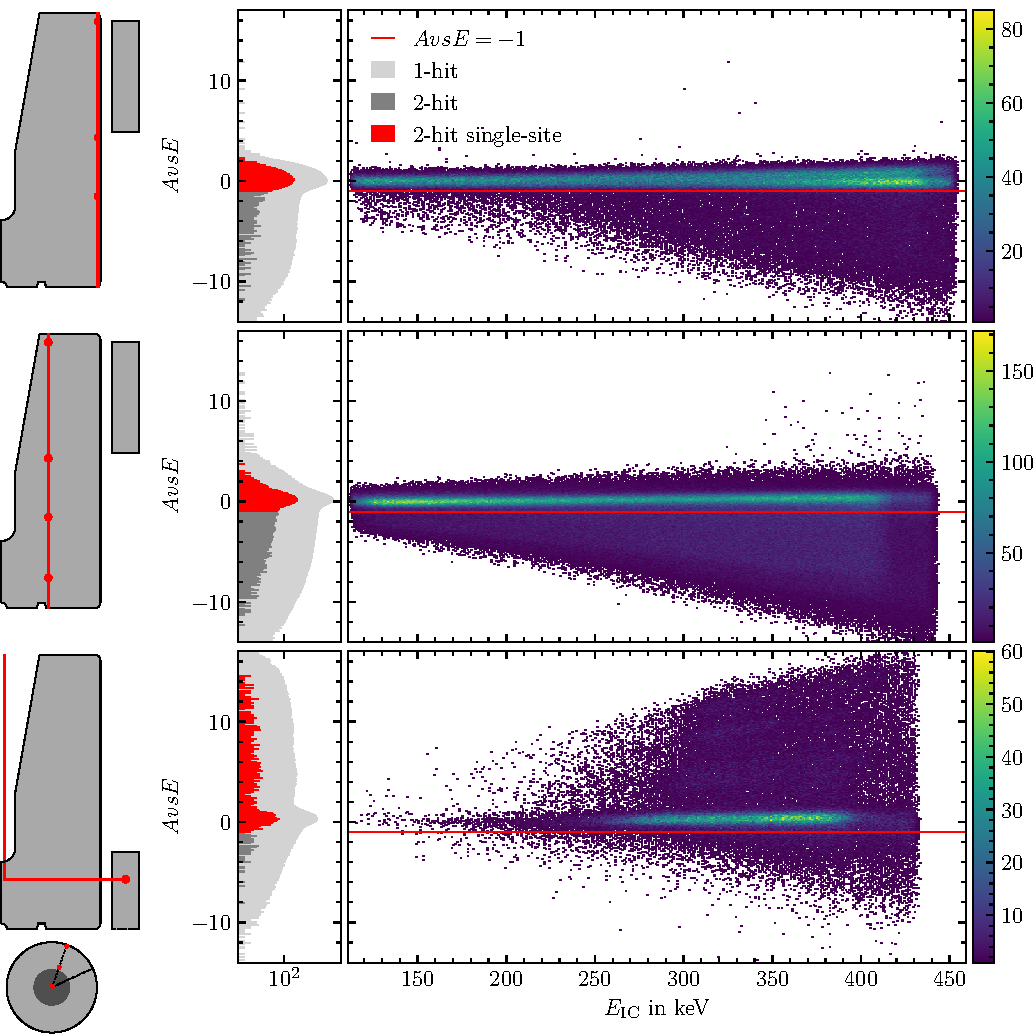
\includegraphics[width=6in]{figs/pipeline/avse_cut_compton.png}
    \caption{$AvsE$ is shown against ICPC energy for $r = (35,17,1)$\,mm for 1-hit events. The corresponding marginalized distributions are shown in light gray on the left. The 2-hit event distributions are included in dark gray, with the accepted single-site population shown in red.}
    \label{fig:avse_compton}
\end{figure}
The Klein-Nishina formula (Eq.~\ref{eq:klein-nishina}) favors forward scattering of 662\,keV gammas, thus detectors with elongated geometries along the gamma beam path, such as the ICPC under study, have a particularly large ratio of multi- to single-site events. This translates into a non-negligible contamination of multi-site events in the 2-hit population. The multi-site contamination increased as the camera was lowered, supporting this conclusion. 

To mitigate the multi-site contamination of 2-hit events, the multi-site event classifier developed in Sec.~\ref{sec:avse} was applied to Compton data. The parameters used to calculate $AvsE$ (Eq.~\ref{eq:avse}) are computed using \ThS{} data, and the cut value $j$ is tuned using the 2-hit events collected with the \CsS{} placed at the outer edge of the detector ($r = 35$\,mm). More concisely, $AvsE$ is tuned such that 94\% of 2-hit events collected at this radius are accepted ($AvsE > -1$). The acceptance was determined empirically, by visual inspection of 1000 of the over 4000 waveforms in this population. The resulting $AvsE$ distribution at this radius and at two others are shown in Fig.~\ref{fig:avse_compton}. $AvsE$ parameter calculation and tuning was conducted separately for soft pileup and resting baseline events, and at the different detector biases, resulting in distinct parameters for each population.

The relative stability of the $AvsE$ mode with respect to $E$ for all radii in Fig.~\ref{fig:avse_compton} demonstrates the correct construction of this parameter. As expected the multi-site contamination is lowest at the outer edge and center of the detector. Also seen in the distribution of the latter, are p$^+$ contact events, characterized by high $AvsE$ values. There is a significant reduction in multi-site contamination in the 2-hit population, as explicitly shown on the right of Fig.~\ref{fig:avse_cam_z} by normalizing the 1-hit and 2-hit distributions for $r = 31$\,mm and the top camera position. 
\begin{figure}[htb]
    \centering
    \includegraphics[width=6in]{figs/pipeline/avse_cam_z.pdf}
    \caption{The normalized $AvsE$ distributions for four camera positions are shown on the left. For the top camera position, the normalized $AvsE$ distribution of all coincident events passing data cleaning cuts is compared with the 1- and 2-hit normalized $AvsE$ distributions.}
    \label{fig:avse_cam_z}
\end{figure}
Also shown on the right of Fig.~\ref{fig:avse_cam_z} is the $AvsE$ distribution for all coincident events that passed data cleaning cuts. This contains all 1-hit, 2-hit and all other events which failed containment and validation cuts. The distributions demonstrate that the $z_\theta$ reconstruction alone already favors single-site events. This is of importance for 1-hit events, which cannot be independently validated, and lends confidence to the quality of the reconstructed $z_\theta$ for this population. On the left of Fig.~\ref{fig:avse_cam_z} the normalized 1-hit event $AvsE$ distributions are shown for all camera positions. It is clear that the multi-site contamination increased as the camera was lowered. 
\begin{figure}[htb]
    \centering
    \includegraphics[width=6in]{figs/pipeline/multisite_contamination.pdf}
    \caption{The 1- and 2-hit multi-site event contamination is shown for data taken at all camera positions at a given radius.}
    \label{fig:multisite_contamination}
\end{figure}

As seen in Fig.~\ref{fig:multisite_contamination}, the 1-hit multi-site contamination ranges from 16\% in outer edge of the detector to 44\% right before the taper edge. From this point inwards, the contamination drops, with a pronounced drop at the borehole edge, as does the thickness of Ge that gammas emitted by the \CsS{} source traverse. The corresponding 2-hit event contaminations are 1.6-3 times lower. 

\section{Self-similarity Cut and 2-hit Superpulses}

Due to the intrinsic resolution of the Compton scanner, a voxel size must be chosen for the pulse shape library. Along with the approximately 2\,mm \CsS{} beam spot diameter, the position reconstruction resolution of 2\,mm provides a natural choice of voxel size: 2\,mm in all spatial dimensions. Starting at $z = 1$\,mm, voxels were created at 2\,mm intervals in $z$, until $z = 99$\,mm for each radial position of the \CsS{} source. A few additional voxels are added at the top and bottom, to confirm that the number of reconstructed events within a voxel fall off rapidly at the detector edges. All the waveforms within a representative sample of voxels were normalized and visually inspected. To perform the normalization, each waveform is divided by its uncalibrated energy. For most of the detector volume, after the application of the $AvsE$ cut, the vast majority of waveforms within a voxel have the same shape. The rare outliers can be attributed to falsely validated events. This statement breaks down in the central region of the detector, where a high weighting potential gradient leads to neighboring voxels with notably different pulse shapes. In such cases, the outliers are most likely spilling over from the neighboring voxels. The 2-hit waveforms that fall in the $(r = 31, z = 11)$\,mm voxel are shown on the left of Fig~\ref{fig:Cs_superpulse_cuts}. 
\begin{figure}[htb]
    \centering
    \includegraphics[width=6in]{figs/pipeline/Cs_superpulse_cuts.pdf}
    \caption{All 2-hits reconstructed for the $(r = 31, z = 11)$\,mm voxel are shown on the left. The successive application of the $AvsE$ and self-similarity cuts retained the events shown in the center and right panels respectively. The number of events, $n$, and the superpulse calculated from the events in each panel are shown.}
    \label{fig:Cs_superpulse_cuts}
\end{figure}

The application of the $AvsE$ classifier removed all but one multi-site event from this population. The events which survived this cut are shown in the middle, with the outlier most likely being the result of an event where most of the energy was deposited at one site, and a second energy deposition caused late collection of charge. This is an example of a falsely validated event that was not caught by the $AvsE$ cut. To remove such outliers a superpulse was constructed by time-aligning and averaging candidate events and applying a self-similarity cut. 

More concisely, only events that are similar to the superpulse -- those with $\chi^2/\text{ndf} \le 3$ -- are retained. Here $\chi^2/\text{ndf}$ is calculated for a waveform with samples $q_i$ as:
\begin{equation}
	\chi^2/\text{ndf} = \frac{1}{300(\sigma_q^2 + \sigma_Q^2)}\sum_{i = -200}^{100}\left(q_i + Q_i\right)^2~,
	\label{eq:chi_sq_wfs}
\end{equation}
where $Q_i$ are the superpulse samples, and $\sigma_q$ and $\sigma_Q$ are the baseline root-mean-square of the waveform and superpulse respectively. In this equation $i=0$ is the point at which waveforms are time-aligned. Along with this point, 200 samples before and 100 samples after this point were used. This forms a 1200\,ns evaluation window for $\chi^2/\text{ndf}$. Although shorter than the maximum simulated drift time, the evaluation window is approximately twice as long as the longest 1-99\% rise time measured in data.  

The superpulse was constructed from the sample-by-sample median of time-aligned waveforms. Just as with the \BaS{} superpulses, the waveforms were time aligned at 50\% of their rise. As can be seen on the left two panels of Fig.~\ref{fig:Cs_superpulse_cuts}, the use of the median minimized the effects of outliers.

Applying the self-similarity cut to the events in the middle panel of Fig.~\ref{fig:Cs_superpulse_cuts} removes the outlier event along with an event with noise on the rising edge, leaving the clean population of events shown on the right. The topology of three of these events is shown in Fig.~\ref{fig:reco_events}.
\begin{figure}[htb]
    \centering
    \includegraphics[width=6in]{figs/pipeline/reco_events.png}
    \caption{Three events reconstructed at the $(r = 31, z = 11)$\,mm voxel.}
    \label{fig:reco_events}
\end{figure}

A final superpulse is created from the events passing the self-similarity cut. The construction of the final 2-hit superpulse differs from that used for the cut. Since no outliers remain, the sample-by-sample weighted average is taken, with the weights corresponding to the calibrated energy calculated for each waveform. 

In voxels with very low statistics say, under 5 events passing the $AvsE$ cut or when more than one clear population is present, the outlier concept is no longer applicable. In such cases the use of the median for the creation of the self-similarity superpulse still favors the population with the greatest number of events. If the number of events is even and there is a clear separation between waveform populations, it is possible for the self-similarity cut to reject all events. For such voxels, the superpulse construction was deemed failed. These cases are relatively rare, and concentrated in the central regions and outside the detector.

\section{Final superpulses}

The 2-hit superpulses contain the most reliable reconstructed data. However, in most cases they are constructed from under 100 waveforms and thus have an appreciable noise-to-signal ratio. The approximately 30 times more numerous 1-hit events can be used to remedy this. To select the correctly reconstructed 1-hit events within a voxel, $\chi^2/\text{ndf}$ is calculated with the voxel's 2-hit superpulse as reference. The $\chi^2/\text{ndf}$ distribution for 1-hit events in the $(r = 31, z = 11)$\,mm voxel is shown on the left of Fig.~\ref{fig:Cs_superpulse_final}.
\begin{figure}[htb]
    \centering
    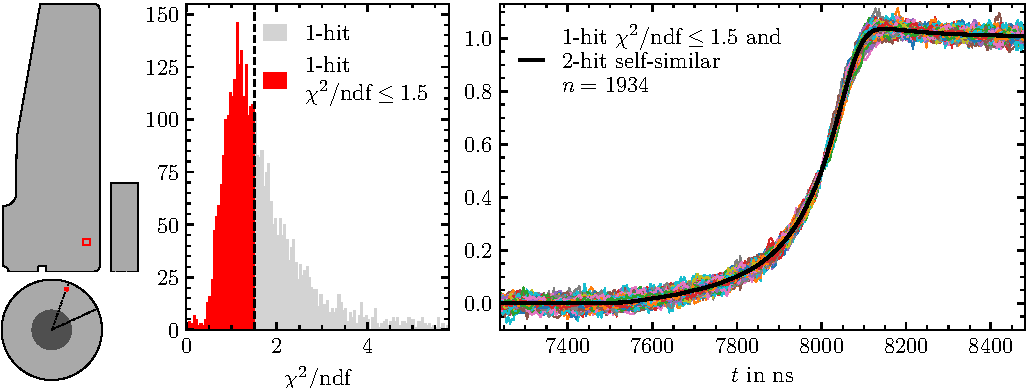
\includegraphics[width=6in]{figs/pipeline/Cs_superpulse_final.png}
    \caption{The $\chi^2/\text{ndf}$ distribution for 1-hit events in the $(r = 31, z = 11)$\,mm voxel is shown in gray on the left. All the waveforms with $\chi^2/\text{ndf} \le 1.5$ are shown on the right, along with 2-hit self-similar waveforms for the same voxel. In conjunction, they are used to create the final superpulse shown in black.}
    \label{fig:Cs_superpulse_final}
\end{figure}

Waveforms with $\chi^2/\text{ndf} \le 1.5$ are selected to join the 2-hit self-similar superpulses in the creation of a final superpulse. The cutoff value was chosen to achieve noise-to-signal ratio of under 0.005 for all superpulses while preserving data quality. Achieving this noise level is of particular importance for the ICPC pulse shape library, since the weighting potential in the upper two thirds of the detector is lower than 0.005. Including 1-hit events results in 1898 additional waveforms for the $(r = 31, z = 11)$\,mm voxel. The resulting superpulse is shown on the right of Fig.~\ref{fig:Cs_superpulse_final}. The construction of the final superpulse follows the procedure employed for the final 2-hit superpulse. Note that for voxels where the 2-hit superpulse construction fails, the addition of 1-hit waveforms cannot be carried out. The final superpulses calculated in the lower half of the detector for $r = 31$\,mm are shown in Fig.~\ref{fig:Cs_superpulse_all_z}.
\begin{figure}[htb]
    \centering
    \includegraphics[width=6in]{figs/pipeline/Cs_superpulse_all_z.pdf}
    \caption{The $(r = 31, z = [1,49])$\,mm superpulses are depicted, with an inset (with matching $x$-scale) showing a close up of the start of the rise. For clarity, superpulses in the top half of the detector are not shown, as they are visually indistinguishable from the $(r = 31, z = 49)$\,mm superpulse (depicted with the brightest color).}
    \label{fig:Cs_superpulse_all_z}
\end{figure}

The procedures outlined in this chapter are applied to all Compton data creating the pulse shape library presented in Chapter~\ref{chap:library}. In most cases the final superpulses have noise-to-signal ratios around or under 0.001. This level of noise allows for the calculation of $t_0$ from superpulses with good accuracy in the lower half of the detector, where the weighing potential is over 0.001.